%!TEX root = ../main.tex

\chapter{Resultados e Discussão} \label{cap:resultados}

Nesta seção serão apresentados os resultados obtidos com o treinamento e teste das arquiteturas canônicas consideradas para este trabalho. As Seções \ref{sec:lenet} e \ref{sec:alexnet} contemplam os resultados obtidos com as arquitetura LeNet e AlexNet, respectivamente, as quais são arquiteturas bem consolidadas no âmbito de \emph{Deep Learning}. Nas Seções \ref{sec:mobilenet}, \ref{sec:shufflenet} e \ref{sec:squeezenet} estão presentes alguns resultados obtidos pelas arquiteturas MobileNet, ShuffleNet e SqueezeNet. Mais adiante, nas Seções \ref{sec:vgg} e \ref{sec:inception}, estão expostos os resultados alcançados pelas CNNs VGG-16 e Inception-V3, as arquiteturas mais profundas escolhidas para este trabalho. O treinamento destas CNNs foi realizado utilizando os recursos computacionais de um servidor, disponível no LSI, dedicado especialmente para tarefas de DL, o qual possui um processador Intel Core i7 com 16 GB de RAM e duas placas gráficas com 11 GB de memória cada, das quais apenas uma foi utilizada.

Após a etapa de treino, foram realizados os testes para aferir os modelos no tocante às métricas de desempenho para o conjunto de testes. Nesta etapa, percebeu-se que alguns modelos tornaram-se degenerados e acabaram prevendo apenas uma das classes. Duas hipóteses podem justificar a ocorrência desse problema: o ReLU \emph{dying problem}, quando a função de ativação ReLU foi utilizada; ou a tendência à permanência em mínimos locais durante o treinamento do modelo. Todas as CNNs que manifestaram este comportamento no conjunto de testes tiveram seus resultados descartados, pois as métricas obtidas não refletiam aprendizado no problema considerado.


\section{Resultados Obtidos com a CNN LeNet}
\label{sec:lenet}
%!TEX root = ../../main.tex


A primeira fase do treinamento dos modelos foi conduzida utilizando a arquitetura LeNet. Nesta fase, foi realizada uma busca em \emph{grid} por todos os hiperparâmetros previamente definidos, conforme Seção \ref{sec:modelos}, e considerando as duas abordagens definidas conforme a Seção \ref{sec:preparacao}, gerando um total de $72$ modelos a serem treinados e testados. Para estes modelos, excluindo aqueles que se tornaram degenerados, utilizou-se a métrica \emph{F-Score} como referência para um melhor desempenho.

O melhor dos modelos baseados na arquitetura LeNet para cada uma das abordagens consideradas encontram-se dispostos na Tabela \ref{tab:lenet}, juntamente com os hiperparâmetros utilizados pelos mesmos.

\begin{table}[h]
\centering
\caption{Detalhamento dos melhores resultados obtidos com a arquitetura LeNet.}
\label{tab:lenet}
\resizebox{\textwidth}{!}{\begin{tabular}{ccccccc}
\toprule
\textbf{Abordagem} & \textbf{Otimizador} & \textbf{\emph{Patience}}  & \textbf{Função de Ativação} & \textbf{Acurácia} & \textbf{\emph{F-Score}} & \textbf{EER} \\
\midrule
Abordagem A & RMSprop & 5 & ReLU & $0.9865$ & $0.9755$ & $1.1679$\\
Abordagem B & Adam & 10 & ELU & $0.8361$ & $0.8159$ & $12.5245$ \\
\bottomrule
\end{tabular}}
\end{table}
\todo{Calcular EER para LeNet}


Os gráficos da Figura \ref{fig:treinamento-lenet} denotam o histórico da perda (\emph{loss}) e acurácia para o conjunto de treinamento e validação destas redes. Nota-se que nenhuma delas chegou ao limite máximo de épocas possíveis, interrompendo o aprendizado por meio de \emph{early stopping}, comportamento este que também fez-se presente em todas as outras redes treinadas com esta arquitetura.

\begin{figure}[h!]
	\centering
	\caption{Histórico de \emph{loss} e acurácia durante o treinamento dos melhores modelos obtidos com a arquitetura LeNet.}
	\subfloat[\emph{Loss} durante treinamento da melhor rede LeNet com a abordagem A.\label{subfig:lenet-a-loss}]{%
	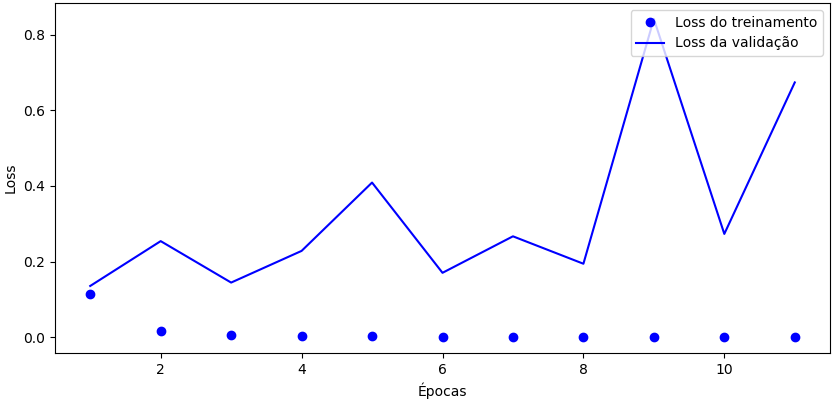
\includegraphics[width=0.45\textwidth]{imgs/lenet-a-loss}
	}
	\hfill
	\subfloat[Acurácia durante treinamento da melhor rede LeNet com a abordagem A.\label{subfig:lenet-a-acc}]{%
	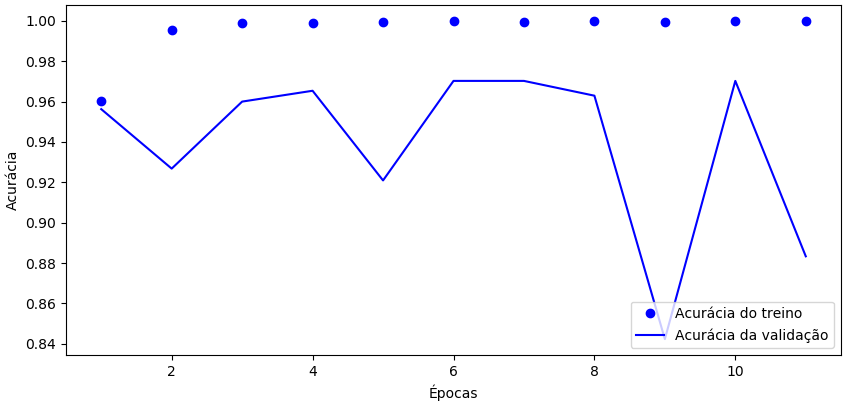
\includegraphics[width=0.45\textwidth]{imgs/lenet-a-acc}
	}
	\hfill
	\subfloat[\emph{Loss} durante treinamento da rede LeNet B.\label{subfig:lenet-b-loss}]{%
	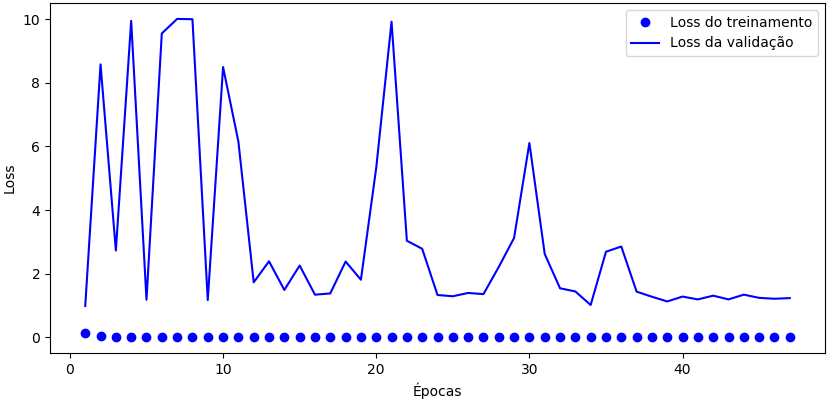
\includegraphics[width=0.45\textwidth]{imgs/lenet-b-loss}
	}
	\hfill
	\subfloat[Acurácia durante treinamento da rede LeNet B.\label{subfig:lenet-b-acc}]{%
	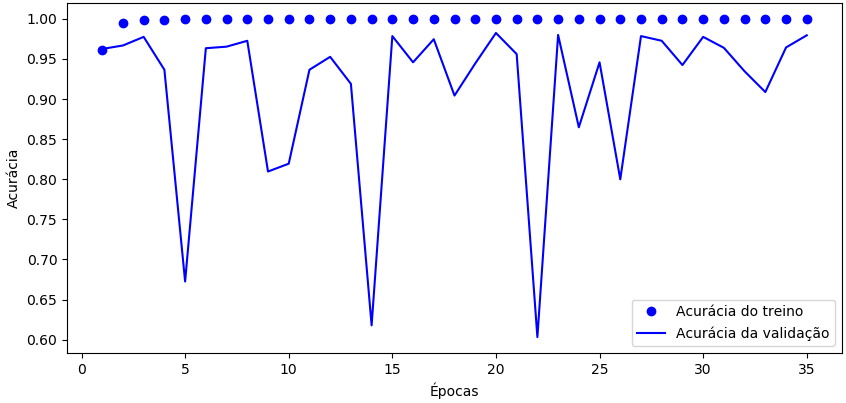
\includegraphics[width=0.45\textwidth]{imgs/lenet-b-acc}
	}
	\label{fig:treinamento-lenet}
\end{figure}

Examinando mais atentamente o desempenho destas redes no conjunto de testes, tem-se, então, as matrizes de confusão mostradas na Figura \ref{fig:matrizes-lenet}. Nestas matrizes, a soma das linhas representam a quantidade de assinaturas previstas para cada classe pelo modelo em questão, enquanto a soma das colunas denotam a quantidade de assinaturas existentes em cada classe.

\begin{figure}[h]
	\centering
	\caption{Matrizes de confusão dos melhores modelos obtidos com a arquitetura LeNet.}\label{fig:matrizes-lenet}
	\subfloat[Melhor LeNet com a abordagem A\label{subfig:matriz-lenet-a}]{%
	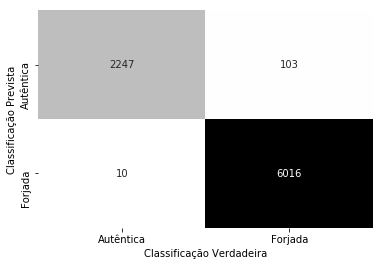
\includegraphics[width=0.47\textwidth]{imgs/matriz-lenet-a}
	}
	\hfill
	\subfloat[Melhor LeNet com a abordagem B\label{subfig:matriz-lenet-b}]{%
	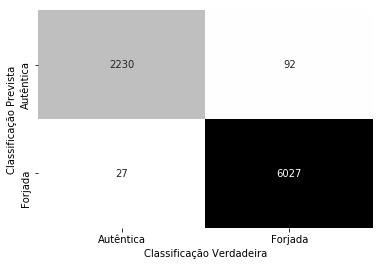
\includegraphics[width=0.47\textwidth]{imgs/matriz-lenet-b}
	}
\end{figure}

%%%% ARGUMENTAÇÃO

Para esta arquitetura, é possível visualizar que, dentre os dois modelos tidos como melhores, não há qualquer semelhança entre os hiperparâmetros encontrados. O número de épocas para aprendizado de características foi baixo para abordagem A, enquanto que, para a abordagem B, houve a necessidade de mais épocas de treinamento. Isso aconteceu, possivelmente, pela aparição de um mesmo autor em partições de dados diferentes na abordagem A.

A partir das matrizes de confusão, percebeu-se que o melhor modelo da abordagem A tendeu a verificar um baixo número de falsos negativos, ou seja, os exemplos autênticos foram suficientes para identificar assinaturas originais, indepentemente das variações cometidas por este autor. Por outro lado, para o modelo da abordagem B, verificou-se um número menor de falsos positivos, validando que, apesar da boa capacidade de certos forjadores \emph{over-the-shoulder} em realizar reproduções verossímeis, este modelo mostrou uma alta competência na detecção deste tipo de assinaturas. Não obstante, nota-se a diagonal principal de ambos os modelos bastante densa, sugerindo uma boa adequação para a tarefa considerada.


\section{Resultados Obtidos com a CNN AlexNet}
\label{sec:alexnet}
%!TEX root = ../../main.tex

%% Trabalhar aqui
Para a AlexNet, assim como para a CNN anterior, foi realizada uma busca em \emph{grid} com os hiperparâmetros selecionados anteriormente, com vistas a obter os melhores modelos para cada abordagem de separação de dados, gerando assim, mais $36$ modelos a serem avaliados quanto às suas métricas de desempenho.

Considerando a métrica de \emph{F-score}, foram selecionados os melhores modelos  desta arquitetura e estes encontram-se listados na Tabela \ref{tab:alexnet}. Na Figura \ref{fig:treinamento-alexnet} pode-se observar os gráficos com os comportamentos dos valores de \emph{loss} e acurácia encontrado nos conjuntos de treinamento e validação durante o estágio de treino destes modelos. Apenas para referência posterior, considerou-se uma rotulação das melhores redes identificadas.

\begin{table}[h!]
\centering
\caption{Detalhamento dos melhores modelos obtidos com a arquitetura AlexNet, organizados de forma decrescente considerando o valor de Acurácia.}
\label{tab:alexnet}
\begin{tabular}{cccccc}
\toprule
\textbf{Identificação} & \textbf{Otimizador} & \textbf{\emph{Patience}}  & \textbf{Função de Ativação} & \textbf{Acurácia} & \textbf{F-Score} \\
\midrule
AlexNet A & Adam & 15 & ELU & $0.9654$ & $0.9393$ \\
AlexNet B & SGD & 10 & \emph{Leaky} ReLU & $0.9601$ & $0.9311$ \\
AlexNet C & SGD & 5 & SELU & $0.9561$ & $0.9244$ \\
\bottomrule
\end{tabular}
\end{table}

\begin{figure}[H]
 \centering
 \caption{Histórico de \emph{loss} e acurácia durante o treinamento dos melhores modelos obtidos com a arquitetura AlexNet.}
 \label{fig:treinamento-alexnet}
 \subfloat[\emph{Loss} durante treinamento da rede AlexNet A.\label{subfig:alexnet-a-loss}]{%
 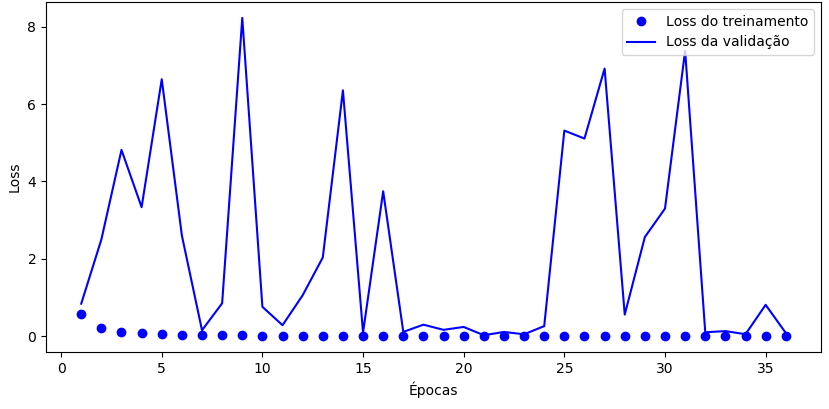
\includegraphics[width=0.45\textwidth]{imgs/alexnet-a-loss}
 }
 \subfloat[Acurácia durante treinamento da rede AlexNet A.\label{subfig:alexnet-a-acc}]{%
 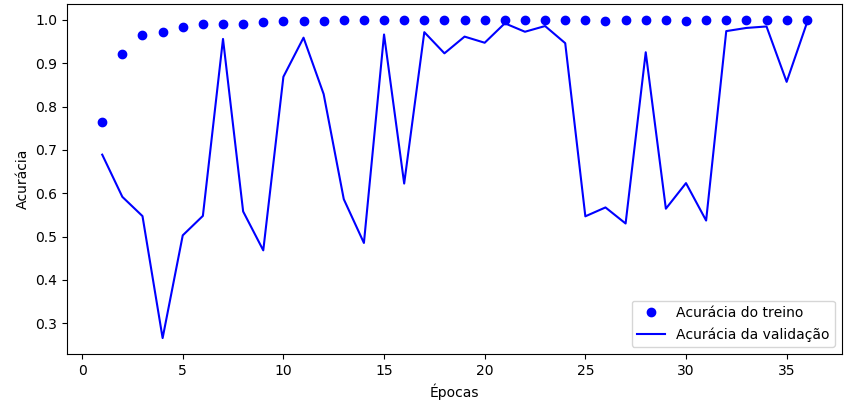
\includegraphics[width=0.45\textwidth]{imgs/alexnet-a-acc}
 }
 \hfill
 \subfloat[\emph{Loss} durante treinamento da rede AlexNet B.\label{subfig:alexnet-b-loss}]{%
 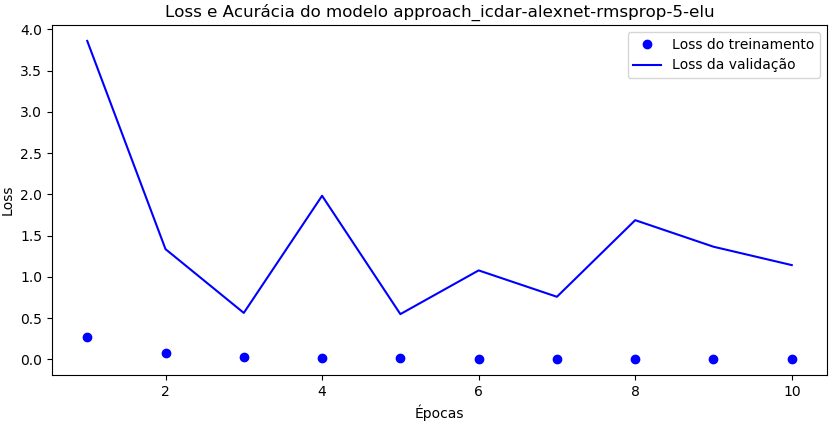
\includegraphics[width=0.45\textwidth]{imgs/alexnet-b-loss}
 }
 \subfloat[Acurácia durante treinamento da rede AlexNet B.\label{subfig:alexnet-b-acc}]{%
 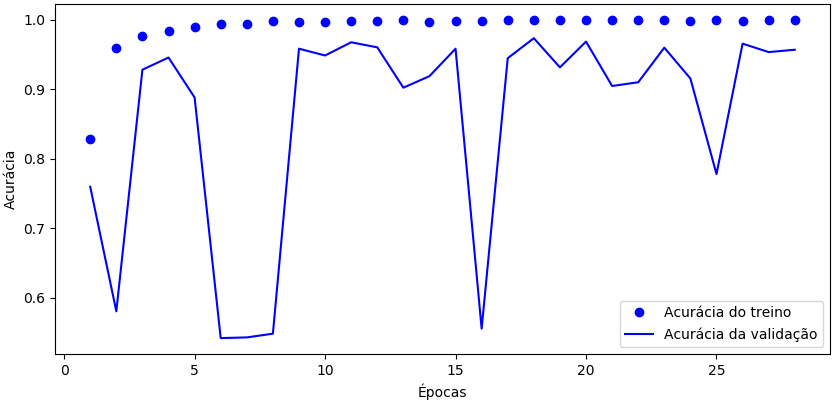
\includegraphics[width=0.45\textwidth]{imgs/alexnet-b-acc}
 }
 \hfill
 \subfloat[\emph{Loss} durante treinamento da rede AlexNet C.\label{subfig:alexnet-c-loss}]{%
 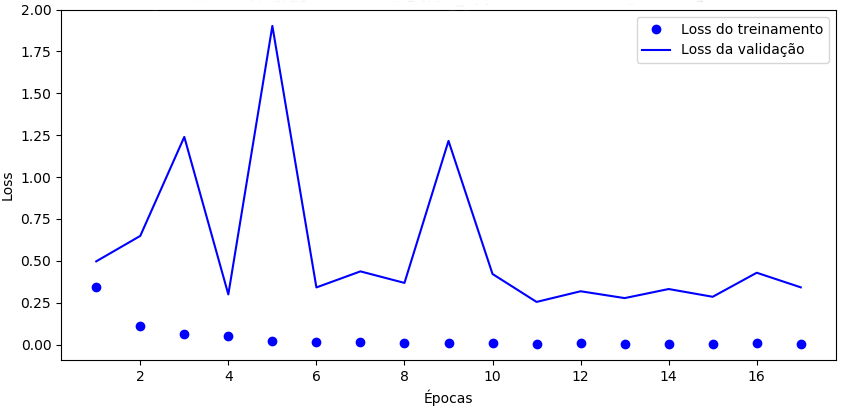
\includegraphics[width=0.45\textwidth]{imgs/alexnet-c-loss}
 }
 \subfloat[Acurácia durante treinamento da rede AlexNet C.\label{subfig:alexnet-c-acc}]{%
 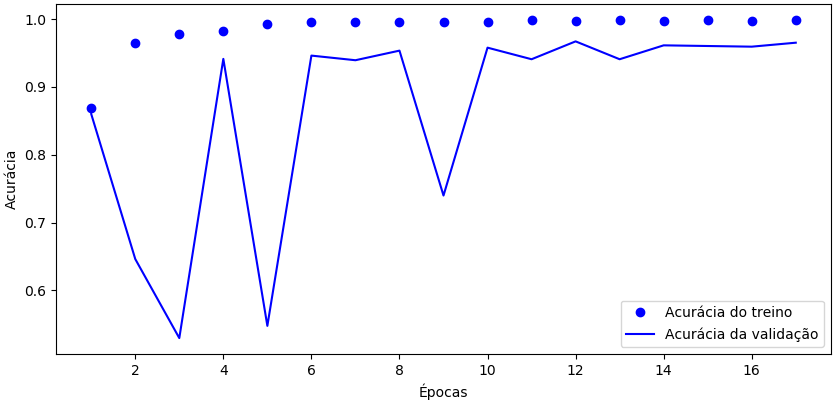
\includegraphics[width=0.45\textwidth]{imgs/alexnet-c-acc}
 }
\end{figure}

Considerando que estas redes possuem mais parâmetros treináveis, este possivelmente foi um fator responsável pelo maior números de épocas no treinamento. Nota-se ainda que houve oscilações nos treinamentos, resultando em parada precoce. Para esta arquitetura, as redes treinadas com otimizador SGD mostraram métricas melhores na etapa de avaliação.

Observando as métricas de acurácia e F-Score obtidas, percebe-se que estas foram inferiores às observadas para as redes LeNet, mas ainda assim alcançando valores superiores a $90\%$. As mesmas reflexões sobre a disposição dos valores na matriz de confusão observados no cenário LeNet se mostram cabíveis, porém com menos acertos.

\begin{figure}[H]
 \centering
 \caption{Matrizes de confusão dos melhores modelos obtidos com a arquitetura AlexNet.}
 \subfloat[AlexNet A\label{subfig:matriz-alexnet-a}]{%
 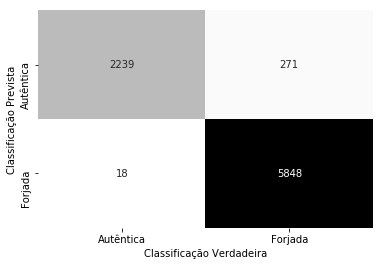
\includegraphics[width=0.5\textwidth]{imgs/matriz-alexnet-a}
 }
 \subfloat[AlexNet B\label{subfig:matriz-alexnet-b}]{%
 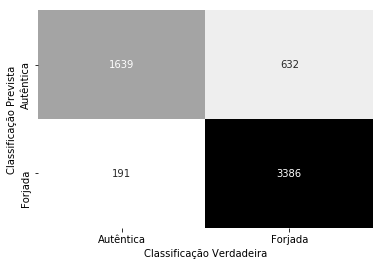
\includegraphics[width=0.5\textwidth]{imgs/matriz-alexnet-b}
 }
 \hfill
 \subfloat[AlexNet C\label{subfig:matriz-alexnet-c}]{%
 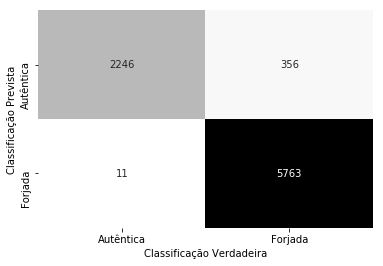
\includegraphics[width=0.5\textwidth]{imgs/matriz-alexnet-c}
 }
 \label{fig:matrizes-alexnet}
\end{figure}

De modo geral, apesar de possuir boas métricas, o melhor modelo encontrado pela arquitetura AlexNet, com um \emph{F-score} de $0.9393$, não foi suficiente para superar o melhor modelo obtido com a arquitetura LeNet ($0.9755$). Uma vez que a arquitetura LeNet possui menos parâmetros que a AlexNet e melhor desempenho observado, ressalta-se a sua maior adequação para a tarefa considerada, acrescido ao fato de demandar menos recursos de tempo de treinamento e de memória para seu armazenamento.


\section{Resultados Obtidos com a CNN MobileNet}
\label{sec:mobilenet}
Seguindo para os resutlados das arquiteturas com poucos parâmetros, a primeira destas a ser treinada e testada foi a MobileNet. Para esta arquitetura, considerando ambas as abordagens, foi realizada mais uma vez uma busca em \emph{grid} de modelos utilizando todos os hiperparâmetros especificados anteriormente, gerando um total de $72$ modelos diferentes.

Nesta arquitetura em particular, foi considerada a métrica de EER para a escolha dos melhores modelos e estes encontram-se presentes na Tabela \ref{tab:mobilenet}. Na Figura \ref{fig:treinamento-mobilenet} pode-se observar os gráficos com o comportamento da \emph{loss} e acurácia dos conjuntos de treino e validação durante a etapa de ajustamento dos modelos.

\begin{table}[h!]
\centering
\caption{Detalhamento dos melhores modelos obtidos com a arquitetura MobileNet para cada uma das abordagens consideradas neste trabalho.}
\label{tab:mobilenet}
\resizebox{\textwidth}{!}{\begin{tabular}{ccccccc}
\toprule
\textbf{Abordagem} & \textbf{Otimizador} & \textbf{\emph{Patience}}  & \textbf{Função de Ativação} & \textbf{Acurácia} & \textbf{F-Score} & \textbf{EER} \\
\midrule
Abordagem A & SGD & 15 & ReLU & $0.9606$ & $0.9318$ & $0.9304$ \\
Abordagem B & Adam & 15 & ReLU & $0.8856$ & $0.8658$ & $9.9475$\\
\bottomrule
\end{tabular}}
\end{table}

\begin{figure}[H]
\centering
\caption{Histórico de \emph{loss} e acurácia durante o treinamento dos melhores modelos obtidos com a arquitetura MobileNet.}
\label{fig:treinamento-mobilenet}
\subfloat[\emph{Loss} durante treinamento da melhor rede MobileNet para a abordagem A.\label{subfig:mobilenet-a-loss}]{%
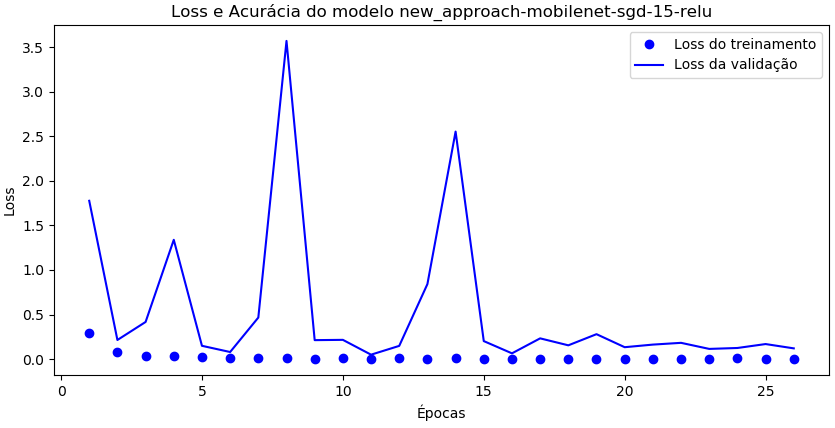
\includegraphics[width=0.47\textwidth]{imgs/mobilenet-a-loss}
}
\hfill
\subfloat[Acurácia durante treinamento da melhor rede MobileNet para a abordagem A.\label{subfig:mobilenet-a-acc}]{%
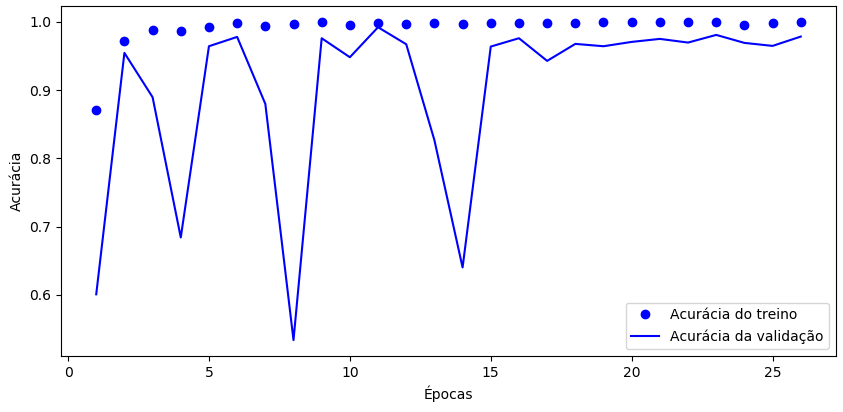
\includegraphics[width=0.47\textwidth]{imgs/mobilenet-a-acc}
}
\hfill
\subfloat[\emph{Loss} durante treinamento da melhor rede MobileNet para a abordagem B.\label{subfig:mobilenet-b-loss}]{%
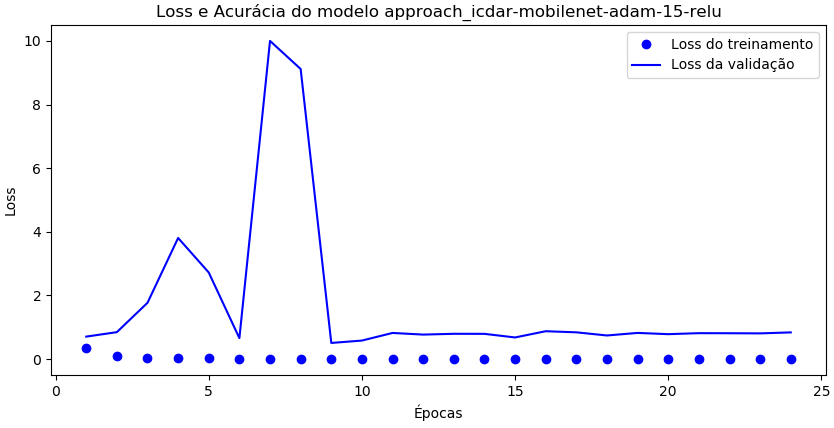
\includegraphics[width=0.47\textwidth]{imgs/mobilenet-b-loss}
}
\hfill
\subfloat[Acurácia durante treinamento da melhor rede MobileNet para a abordagem B.\label{subfig:mobilenet-b-acc}]{%
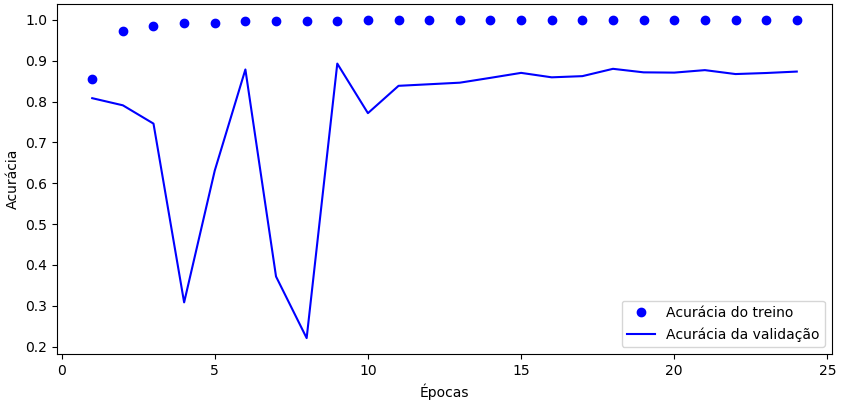
\includegraphics[width=0.47\textwidth]{imgs/mobilenet-b-acc}
}
\end{figure}

Dentre as CNNs observadas até o momento, a MobileNet foi a que obteve um melhor desempenho. Isso se deve, possivelmente, aos poucos padrões encontrados nas imagens de treinamento, por se tratar de imagens em escala de cinza, e à existência de poucos parâmetros treináveis para esta arquitetura. Essas duas características se fizeram essenciais para a descoberta de modelos superiores aos demais, quando analisando apenas a métrica de EER.

Na Figura \ref{fig:matrizes-mobilenet} pode-se visualizar as matrizes de confusão obtidas pelos melhores modelos. Percebe-se que, para abordagem A, apesar da diagonal principal densa, a quantidade de falsos negativos foi maior do que o encontrado nas arquiteturas anteriores para a mesma abordagem. Quanto à matriz encontrada para a abordagem B, podemos considerar as mesmas reflexões concebidas à matriz da arquitetura LeNet.

\begin{figure}[h]
	\centering
	\caption{Matrizes de confusão dos melhores modelos obtidos com a arquitetura MobileNet.}\label{fig:matrizes-mobilenet}
	\subfloat[Melhor MobileNet com a abordagem A\label{subfig:matriz-mobilenet-a}]{%
	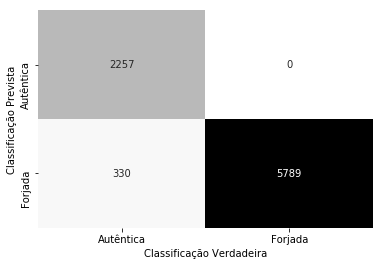
\includegraphics[width=0.47\textwidth]{imgs/matriz-mobilenet-a}
	}
	\hfill
	\subfloat[Melhor MobileNet com a abordagem B\label{subfig:matriz-mobilenet-b}]{%
	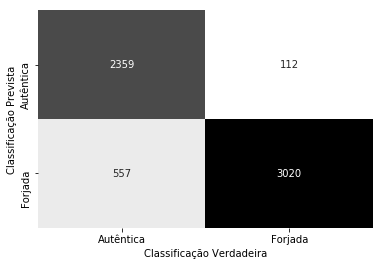
\includegraphics[width=0.47\textwidth]{imgs/matriz-mobilenet-b}
	}
\end{figure}

\section{Resultados Obtidos com a CNN ShuffleNet}
\label{sec:shufflenet}
\begin{table}[h!]
\centering
\caption{Detalhamento dos modelos obtidos com a arquitetura ShuffleNet para cada uma das abordagens consideradas neste trabalho.}
\label{tab:shufflenet}
\resizebox{\textwidth}{!}{\begin{tabular}{ccccccc}
\toprule
\textbf{Abordagem} & \textbf{Otimizador} & \textbf{\emph{Patience}}  & \textbf{Função de Ativação} & \textbf{Acurácia} & \textbf{F-Score} & \textbf{EER} \\
\midrule
Abordagem A & RMSprop & 15 & ReLU & $0.9404$ & $0.9004$ & $7.5400$ \\
Abordagem B & RMSprop & 15 & ReLU & $0.8345$ & $0.7705$ & $23.8151$\\
\bottomrule
\end{tabular}}
\end{table}
    
\begin{figure}[H]
\centering
\caption{Histórico de \emph{loss} e acurácia durante o treinamento dos modelos obtidos com a arquitetura ShuffleNet.}
\label{fig:treinamento-shufflenet}
\subfloat[\emph{Loss} durante treinamento da rede ShuffleNet para a abordagem A.\label{subfig:shufflenet-a-loss}]{%
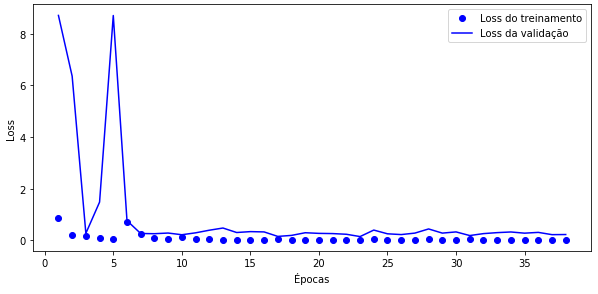
\includegraphics[width=0.47\textwidth]{imgs/shufflenet-a-loss}
}
\hfill
\subfloat[Acurácia durante treinamento da rede ShuffleNet para a abordagem A.\label{subfig:shufflenet-a-acc}]{%
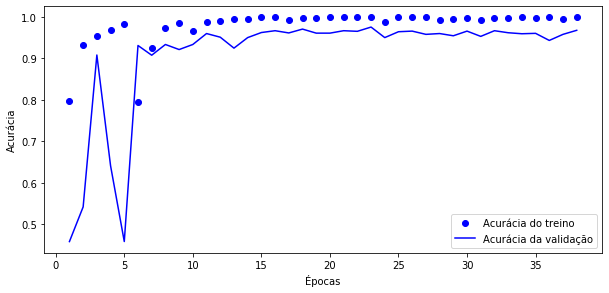
\includegraphics[width=0.47\textwidth]{imgs/shufflenet-a-acc}
}
\hfill
\subfloat[\emph{Loss} durante treinamento da rede ShuffleNet para a abordagem B.\label{subfig:shufflenet-b-loss}]{%
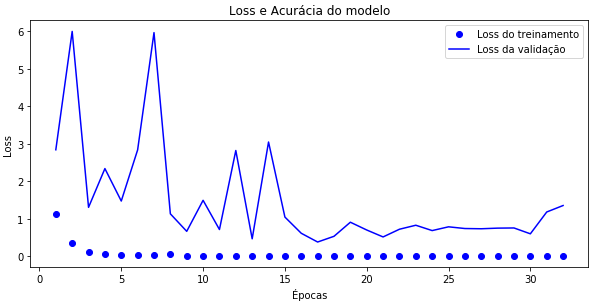
\includegraphics[width=0.47\textwidth]{imgs/shufflenet-b-loss}
}
\hfill
\subfloat[Acurácia durante treinamento da rede ShuffleNet para a abordagem B.\label{subfig:shufflenet-b-acc}]{%
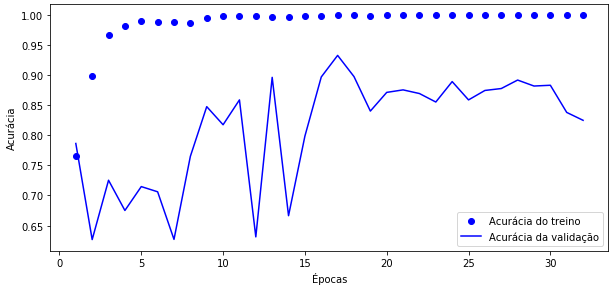
\includegraphics[width=0.47\textwidth]{imgs/shufflenet-b-acc}
}
\end{figure}
    
\begin{figure}[h]
    \centering
    \caption{Matrizes de confusão dos modelos obtidos com a arquitetura ShuffleNet.}\label{fig:matrizes-shufflenet}
    \subfloat[ShuffleNet com a abordagem A\label{subfig:matriz-shufflenet-a}]{%
    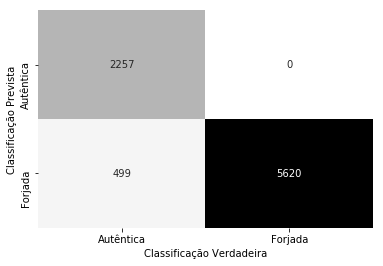
\includegraphics[width=0.47\textwidth]{imgs/matriz-shufflenet-a}
    }
    \hfill
    \subfloat[ShuffleNet com a abordagem B\label{subfig:matriz-shufflenet-b}]{%
    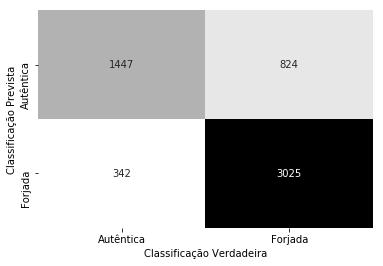
\includegraphics[width=0.47\textwidth]{imgs/matriz-shufflenet-b}
    }
\end{figure}

\section{Resultados Obtidos com a CNN SqueezeNet}
\label{sec:squeezenet}
\begin{table}[h!]
\centering
\caption{Detalhamento dos modelos obtidos com a arquitetura SqueezeNet para cada uma das abordagens consideradas neste trabalho.}
\label{tab:squeezenet}
\resizebox{\textwidth}{!}{\begin{tabular}{ccccccc}
\toprule
\textbf{Abordagem} & \textbf{Otimizador} & \textbf{\emph{Patience}}  & \textbf{Função de Ativação} & \textbf{Acurácia} & \textbf{F-Score} & \textbf{EER} \\
\midrule
Abordagem A & RMSprop & 15 & ReLU & $0.9048$ & $0.8948$ & $11.5074$ \\
Abordagem B & RMSprop & 15 & ReLU & $0.8210$ & $0.7709$ & $20.1673$\\
\bottomrule
\end{tabular}}
\end{table}
    
\begin{figure}[H]
\centering
\caption{Histórico de \emph{loss} e acurácia durante o treinamento dos modelos obtidos com a arquitetura SqueezeNet.}
\label{fig:treinamento-squeezenet}
\subfloat[\emph{Loss} durante treinamento da rede SqueezeNet para a abordagem A.\label{subfig:squeezenet-a-loss}]{%
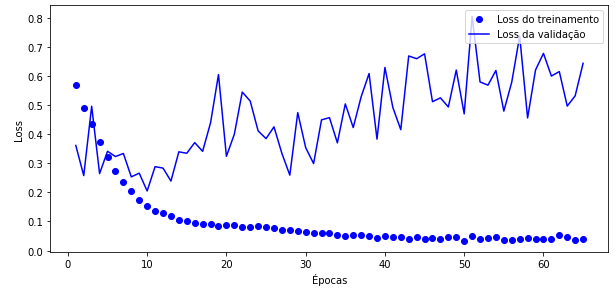
\includegraphics[width=0.47\textwidth]{imgs/squeezenet-a-loss}
}
\hfill
\subfloat[Acurácia durante treinamento da rede SqueezeNet para a abordagem A.\label{subfig:squeezenet-a-acc}]{%
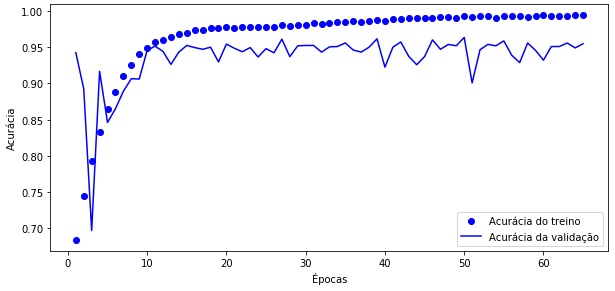
\includegraphics[width=0.47\textwidth]{imgs/squeezenet-a-acc}
}
\hfill
\subfloat[\emph{Loss} durante treinamento da rede SqueezeNet para a abordagem B.\label{subfig:squeezenet-b-loss}]{%
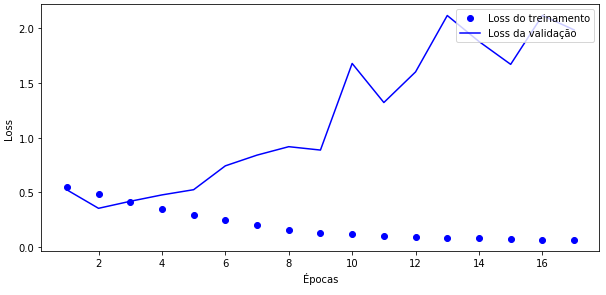
\includegraphics[width=0.47\textwidth]{imgs/squeezenet-b-loss}
}
\hfill
\subfloat[Acurácia durante treinamento da rede SqueezeNet para a abordagem B.\label{subfig:squeezenet-b-acc}]{%
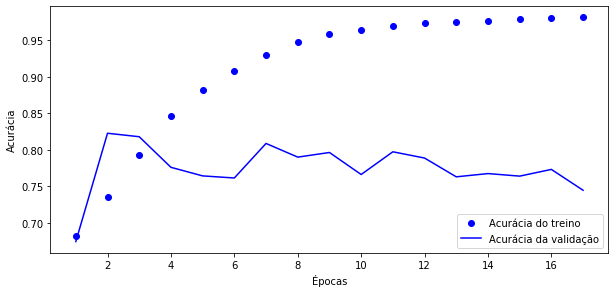
\includegraphics[width=0.47\textwidth]{imgs/squeezenet-b-acc}
}
\end{figure}
    
\begin{figure}[h]
    \centering
    \caption{Matrizes de confusão dos modelos obtidos com a arquitetura SqueezeNet.}\label{fig:matrizes-squeezenet}
    \subfloat[SqueezeNet com a abordagem A\label{subfig:matriz-squeezenet-a}]{%
    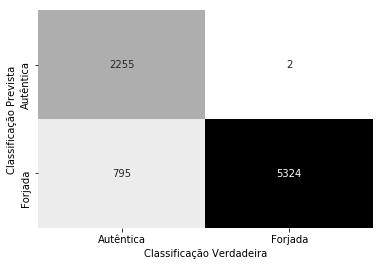
\includegraphics[width=0.47\textwidth]{imgs/matriz-squeezenet-a}
    }
    \hfill
    \subfloat[SqueezeNet com a abordagem B\label{subfig:matriz-squeezenet-b}]{%
    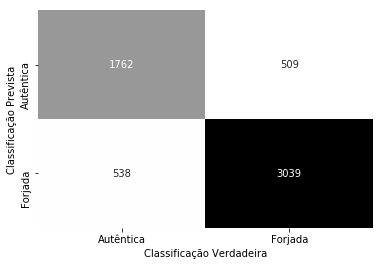
\includegraphics[width=0.47\textwidth]{imgs/matriz-squeezenet-b}
    }
\end{figure}

\section{Resultados Obtidos com a CNN VGG-16}
\label{sec:vgg}
\begin{table}[h!]
\centering
\caption{Detalhamento do modelo obtido com a arquitetura VGG-16 para a abordagem B.}
\label{tab:shufflenet}
\begin{tabular}{cccccc}
\toprule
\textbf{Otimizador} & \textbf{\emph{Patience}}  & \textbf{Função de Ativação} & \textbf{Acurácia} & \textbf{F-Score} & \textbf{EER} \\
\midrule
RMSprop & 10 & ELU & $0.8391$ & $0.8019$ & $16.1096$ \\
\bottomrule
\end{tabular}
\end{table}

\begin{figure}[H]
\centering
\caption{Histórico de \emph{loss} e acurácia durante o treinamento do modelo obtido com a arquitetura VGG-16.}
\label{fig:treinamento-vgg}
\subfloat[\emph{Loss} durante treinamento da rede VGG-16 para a abordagem B.\label{subfig:vgg-b-loss}]{%
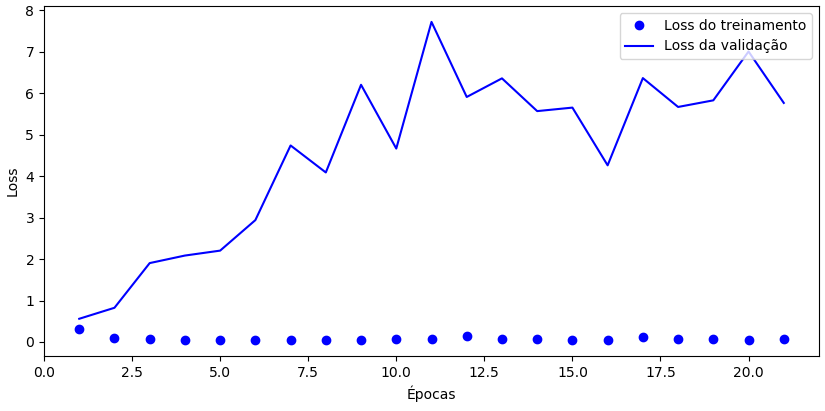
\includegraphics[width=0.47\textwidth]{imgs/vgg-b-loss}
}
\hfill
\subfloat[Acurácia durante treinamento da rede VGG-16 para a abordagem B.\label{subfig:vgg-b-acc}]{%
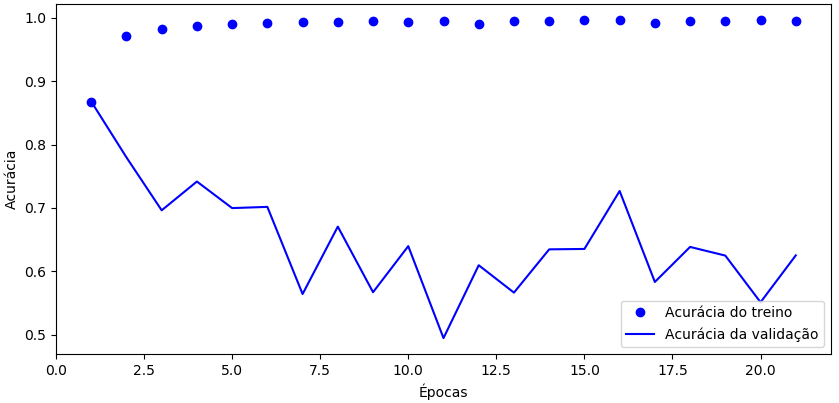
\includegraphics[width=0.47\textwidth]{imgs/vgg-b-acc}
}
\end{figure}

\begin{figure}[h]
    \centering
    \caption{Matriz de confusão do modelo obtido com a arquitetura VGG-16.}\label{fig:matrizes-vgg}
    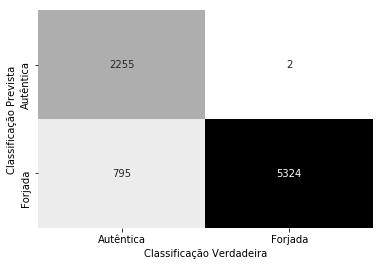
\includegraphics[width=0.6\textwidth]{imgs/matriz-squeezenet-a}
\end{figure}

\section{Resultados Obtidos com a CNN Inception-V3}
\label{sec:inception}
Seguindo para a última das arquiteturas de CNNs exploradas neste trabalho, temos a Inception-V3. Como na CNN anterior, foi treinado apenas um modelo com a abordagem B, a qual se aplicam as mesmas justificativas para tal.

Os hiperparâmetros, definidos de forma arbitrária, e as métricas obtidas para este modelo encontram-se na Tabela \ref{tab:inception}. Uma visualização da \emph{loss} e acurácia durante o treinamento estão caracterizados na Figura \ref{fig:treinamento-inception}.

\begin{table}[h!]
\centering
\caption{Detalhamento do modelo obtido com a arquitetura Inception-V3 para a abordagem B.}
\label{tab:inception}
\begin{tabular}{cccccc}
\toprule
\textbf{Otimizador} & \textbf{\emph{Patience}}  & \textbf{Função de Ativação} & \textbf{Acurácia} & \textbf{F-Score} & \textbf{EER} \\
\midrule
RMSprop & 5 & ELU & $0.8394$ & $0.8070$ & $16.9493$ \\
\bottomrule
\end{tabular}
\end{table}

\begin{figure}[H]
\centering
\caption{Histórico de \emph{loss} e acurácia durante o treinamento do modelo obtido com a arquitetura Inception-V3.}
\label{fig:treinamento-inception}
\subfloat[\emph{Loss} durante treinamento da rede Inception-V3 para a abordagem B.\label{subfig:inception-b-loss}]{%
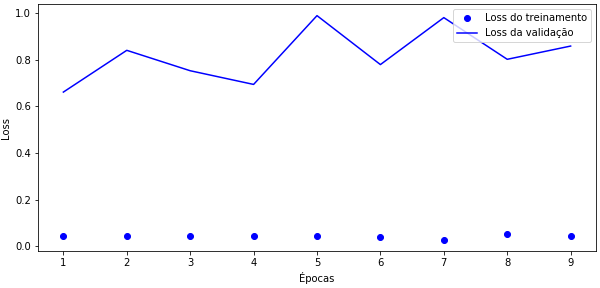
\includegraphics[width=0.47\textwidth]{imgs/inception-b-loss}
}
\hfill
\subfloat[Acurácia durante treinamento da rede Inception-V3 para a abordagem B.\label{subfig:inception-b-acc}]{%
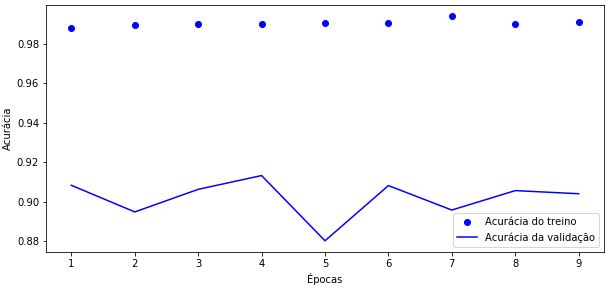
\includegraphics[width=0.47\textwidth]{imgs/inception-b-acc}
}
\end{figure}

É possível examinar a parada precoce do treinamento, levando apenas $9$ épocas antes de chegar ao final. Isto se deve, provavelmente, à capacidade da Inception de detectar os padrões das imagens, o que pode levar a um \emph{overfitting} ao conjunto de treinamento que, consequentemente, diminui o valor da acurácia no conjunto de validação.

A matriz de confusão exibida na Figura \ref{fig:matrizes-inception} diz respeito ao modelo treinado com esta arquitetura. Tem-se um resultado similar ao observado na arquitetura VGG-16, portanto, cabem aqui as mesmas ponderações demonstradas anteriormente.

\begin{figure}[h]
    \centering
    \caption{Matriz de confusão do modelo obtido com a arquitetura Inception-V3.}\label{fig:matrizes-inception}
    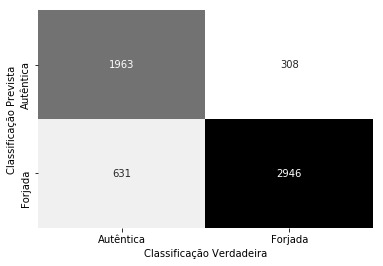
\includegraphics[width=0.6\textwidth]{imgs/matriz-inception}
\end{figure}

Por fim, foi possível comprovar que esta arquitetura consegue prestigiar nosso problema com resultados satisfatórios. Porém, novamente, fica aberta a reflexão sobre a necessidade da utilização de uma arquitetura tão profunda para tratar um problema que foi adequadamente ajustado por CNNs mais rasas. Não obstante, pode ser realizada uma busca exploratória sobre os hiperparâmetros, com vistas à descoberta de resultados superiores aos observados nestas arquiteturas rasas.